%%
%  ******************************************************************************
%  * #file    Szablon_raportu_EN_Latex.tex
%  * #author  Adrian Wójcik   adrian.wojcik(at)put.poznan.pl
%  *          
%  * #commit  Patryk Kościk   koscikpatryk(at)gmail.com
%  *          Modified the template for Projekt przejsciowy purposes          
%  *          
%  *
%  * #commit  Patryk Kościk   koscikpatryk(at)gmail.com
%  *          Zupełnie przewrócono na łeb formatke po taktycznym wyjasnieniu          
%  *          
%  * #version 1.1
%  * #date    09-Mar-2022
%  * #brief   PROJPRZEJ
%  *
%  ******************************************************************************
%%  
\documentclass[11pt, a4paper]{article}

\usepackage{SM_template}

% Wypełnijcie te dyrektywy zgodnie z waszym tematem
%
% \lab      -> NAZWA CZUJNIKA,          np.: 'DHT22'
% \comment  -> Króciutki opis co to,    np.: 'Cyfrowy czujnik temperatury'
% \author   -> Autor dokumentu          np.: Patryk Kościk
%
% Pamiętajcie o zmianie ścieżki w \addbibresourcue (!)

\lab{Moduł KY-038}
\comment{Mikrofon}
\author{Dawid Włodarczyk}
\addbibresource{bib/KY-038.bib}
\nocite{*}
%
% Początek dokumentu
%
\begin{document}

%
% Strona tytułowa
%
\mainpage{KY-038/ky038.jpeg}
\newpage

\section*{Opis elementu}
Mikrofon możemy wykorzystać do wykrywania różnych dźwięków, np. trzaśnięcie drzwiami bądź dmuchanie ustami. Czujnik posiada wyjście zarówno analogowe jak i cyfrowe, więc możliwe jest sterowanie róznymi mikroprocesorami. 
%%%%%%%%%%%%%%%%%%%%%%%%%  TWO IMAGES SIDE BY SIDE  %%%%%%%%%%%%%%%%%%%%%%%%%%%%%
\vspace{0.25cm}
\begin{figure}[h]
\centering
%%%%%%%%%%%%%%%%%%%%%%%%%%%%%%%%%%%%%%%%%%%%%%%%%%%%%%%%%%%%%%%%%%%%%%%%%%%%%%%%%
\begin{subfigure}{.5\textwidth}
\centering
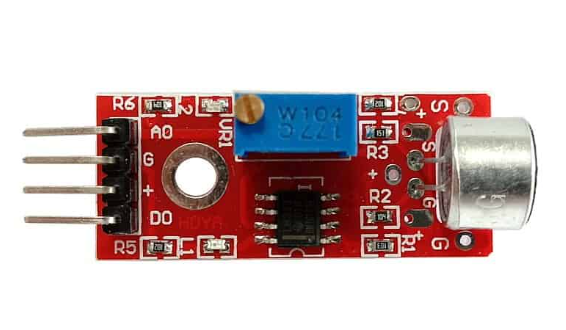
\includegraphics[width=.7\linewidth]{fig/KY-038/zasada_dzialania/front_mikro.png}
\caption{Widok na przód mikrofonu \cite{przod}}
\label{fig:_zdjecie_elementu}
\end{subfigure}%
%%%%%%%%%%%%%%%%%%%%%%%%%%%%%%%%%%%%%%%%%%%%%%%%%%%%%%%%%%%%%%%%%%%%%%%%%%%%%%%%%
\begin{subfigure}{.5\textwidth}
\centering
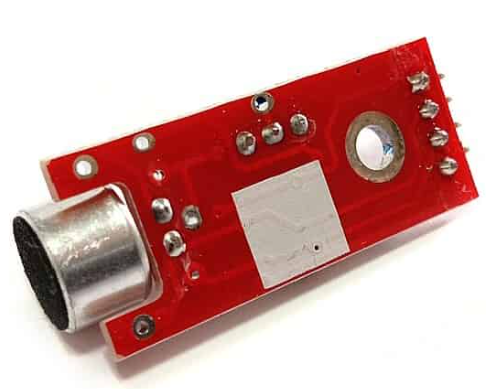
\includegraphics[width=.6\linewidth]{fig/KY-038/zasada_dzialania/tyl_mikro.png}
\caption{Widok na tył mikrofonu \cite{tyl}}
\label{fig:_zasada_dzialania_elementu}
\end{subfigure}
%%%%%%%%%%%%%%%%%%%%%%%%%%%%%%%%%%%%%%%%%%%%%%%%%%%%%%%%%%%%%%%%%%%%%%%%%%%%%%%%%
% \caption{PODPIS}
\label{fig:element}
\end{figure}
\vspace{0.25cm}
%%%%%%%%%%%%%%%%%%%%%%%%%  TWO IMAGES SIDE BY SIDE  %%%%%%%%%%%%%%%%%%%%%%%%%%%%%



% \subsection{Opis modułu} REPLACE SUBSECTION WITH 1CM VSPACE
\vspace{0.75cm}
Wyjście analogowe zapewnia rzeczywisty w czasie pomiar woltażu sygnału na mikrofonie, natomiast w wyjście cyfrowe wyprowadza sygnał wysoki w momencie przekroczenia przez dźwięk odpowiedniego progu. Czujnik może być zasilany 3.3V/5V, posiada 2 diody (jedna sygnalizuje przepływ prądu, druga pojawienie się informacji na wyjściu). Wbudowany jest także potencjometr, którym możemy ustawić wartość progu dźwięku. 

%%%%%%%%%%%%%%%%%%%%%%%%%  TWO IMAGES SIDE BY SIDE  %%%%%%%%%%%%%%%%%%%%%%%%%%%%%
\begin{figure}[h]
\centering
%%%%%%%%%%%%%%%%%%%%%%%%%%%%%%%%%%%%%%%%%%%%%%%%%%%%%%%%%%%%%%%%%%%%%%%%%%%%%%%%%
\begin{subfigure}{.5\textwidth}
\centering
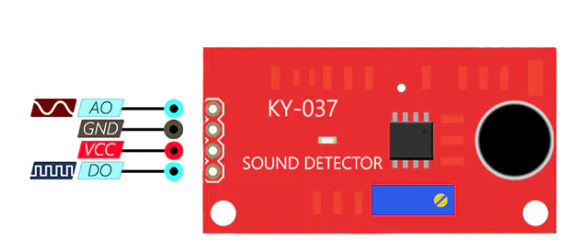
\includegraphics[width=.8\linewidth]{fig/KY-038/zasada_dzialania/uklad.png}
\caption{Elementy układu \cite{modul}}
\label{fig:_zdjecie_modulu}
\end{subfigure}%
%%%%%%%%%%%%%%%%%%%%%%%%%%%%%%%%%%%%%%%%%%%%%%%%%%%%%%%%%%%%%%%%%%%%%%%%%%%%%%%%%
\begin{subfigure}{.5\textwidth}
\centering
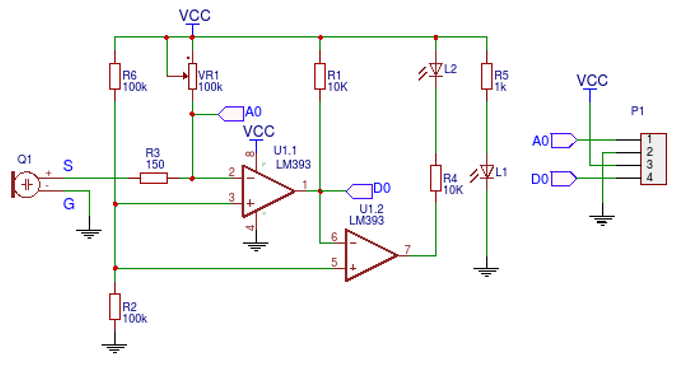
\includegraphics[width=.8\linewidth]{fig/KY-038/zdj_modułu/schemat_mikro.png}
\caption{Schemat modułu \cite{schemat}}
\label{fig:_schemat_modulu}
\end{subfigure}
%%%%%%%%%%%%%%%%%%%%%%%%%%%%%%%%%%%%%%%%%%%%%%%%%%%%%%%%%%%%%%%%%%%%%%%%%%%%%%%%%
\label{fig:modul}
\end{figure}
\vspace{0.5cm}
%%%%%%%%%%%%%%%%%%%%%%%%%  TWO IMAGES SIDE BY SIDE  %%%%%%%%%%%%%%%%%%%%%%%%%%%%%

Jednym z możliwych zastosowań mikrofonu jest zamontowanie go np. w kamerze, która będzie monitorować zmiany terenu oraz rejestrować pojawiające się w terenie dźwięki. 
\newline
Ogólny schemat elektryczny modułu KY-038 przedstawiono powyżej (\ref{fig:_schemat_modulu}).

\newpage

\section{Użycie czujnika}

\vspace{0.25cm}

\begin{figure}[H]
    \centering
    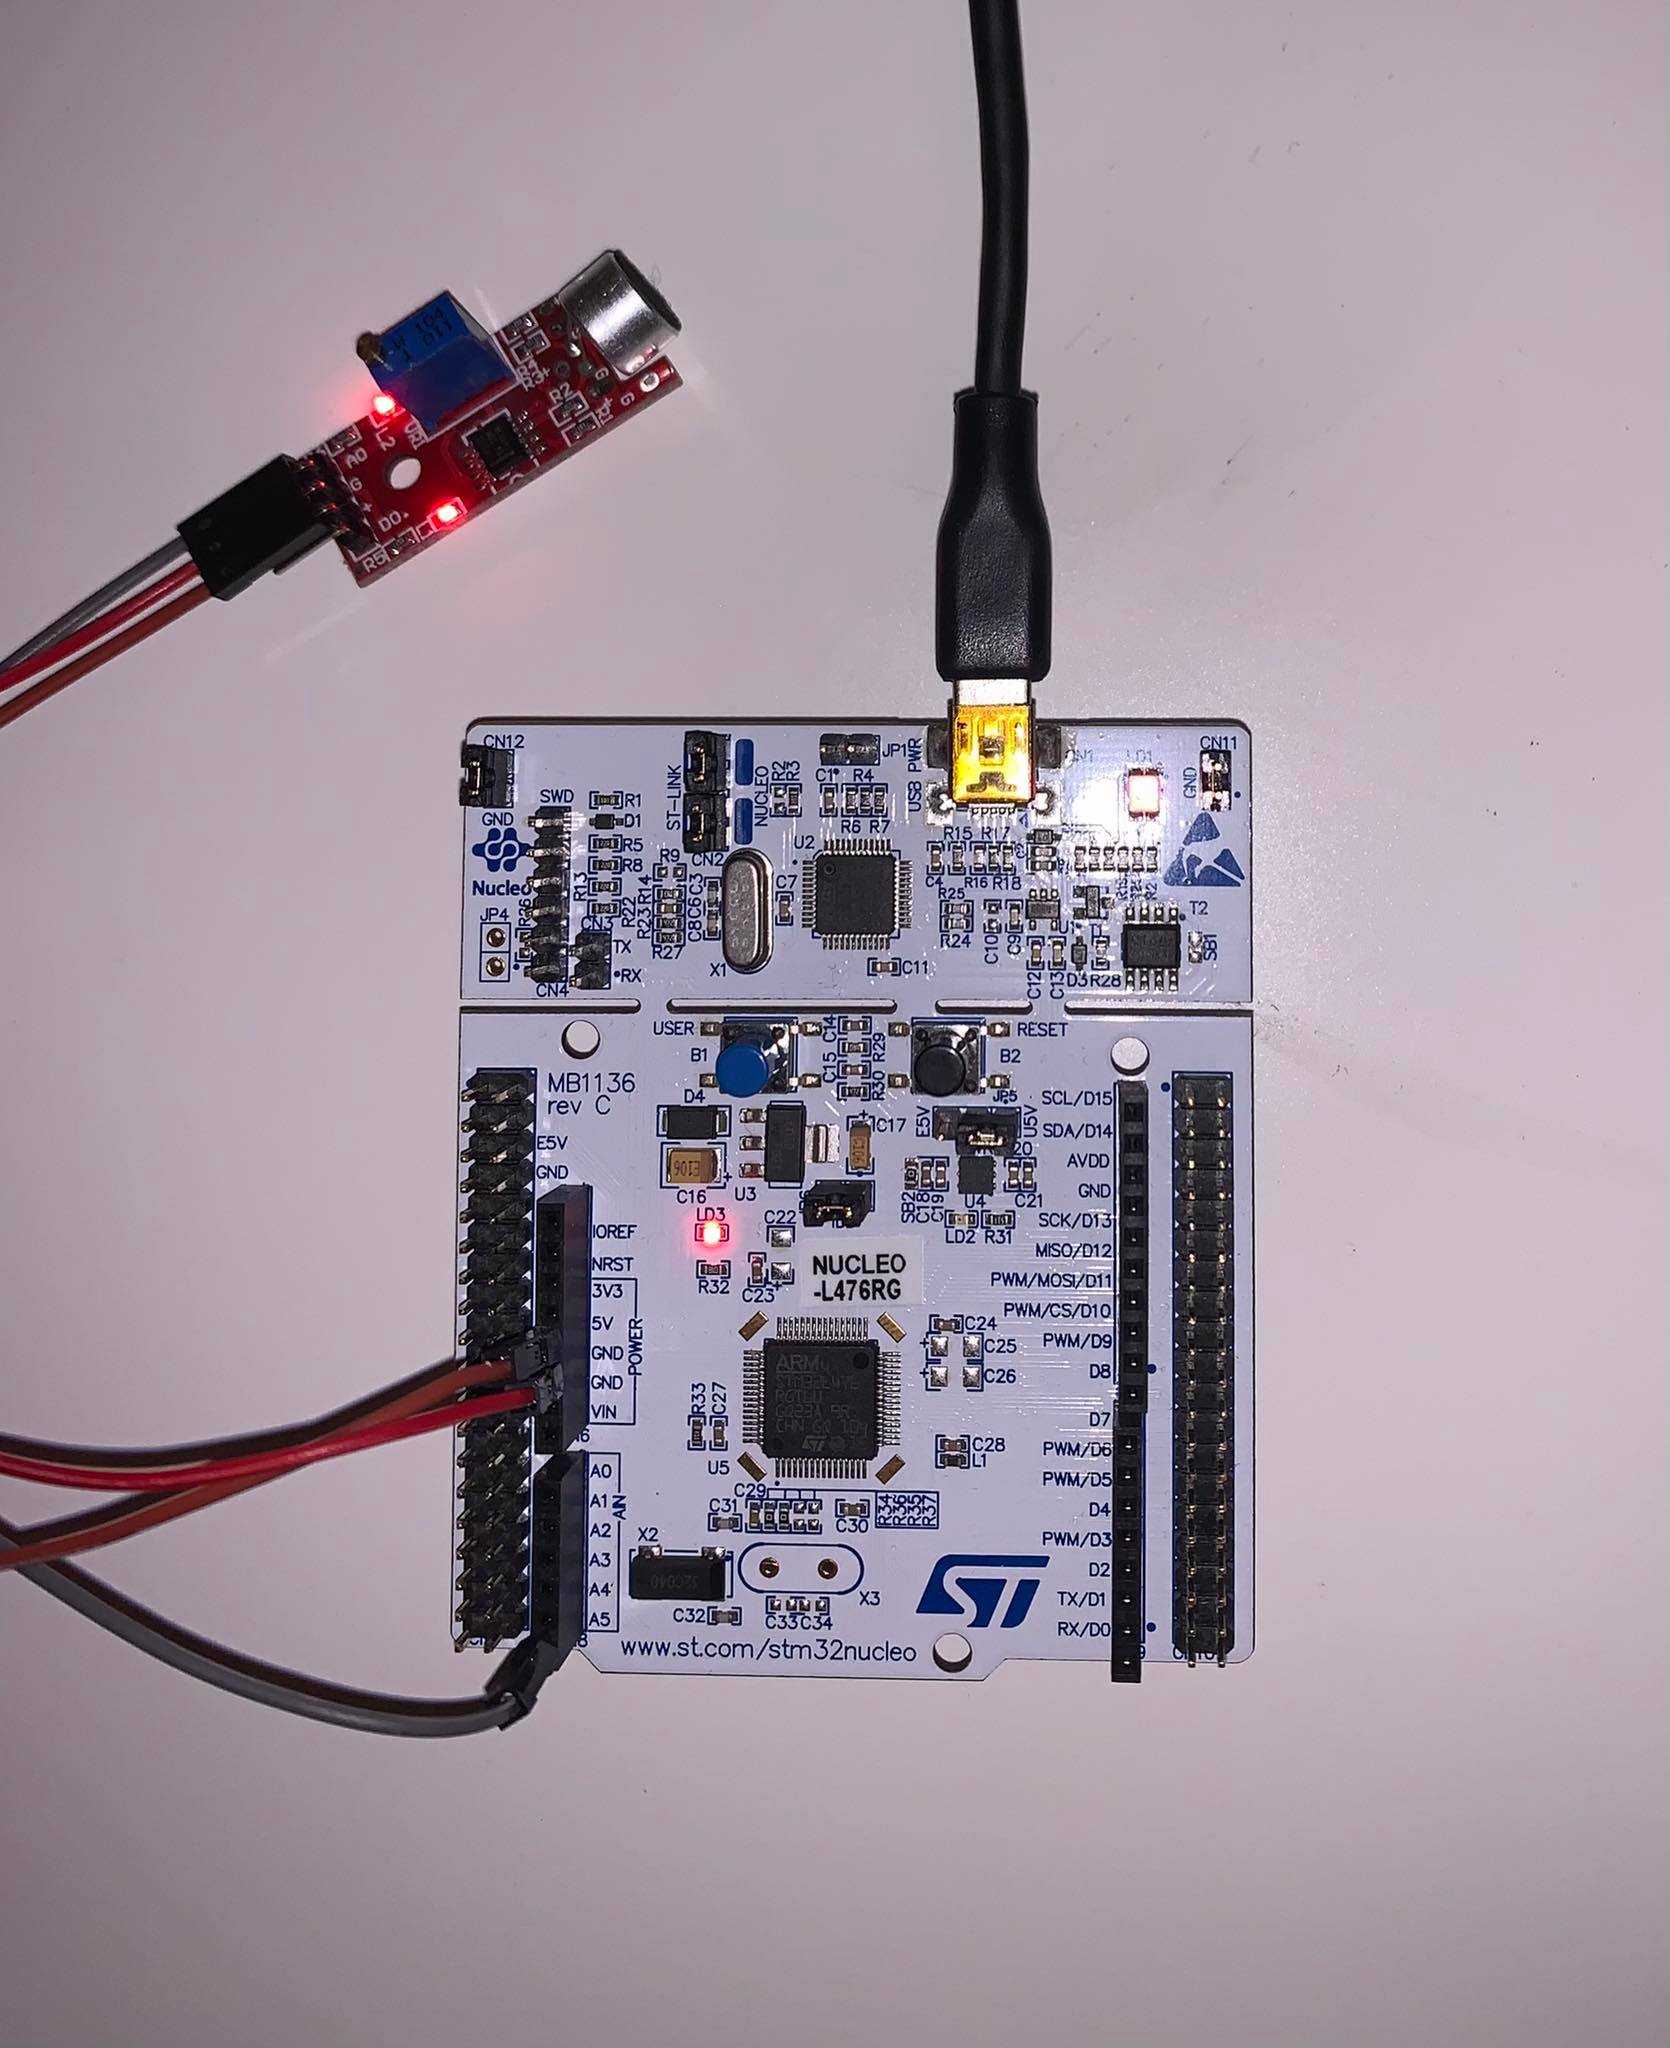
\includegraphics[scale=0.25]{fig/KY-038/zdj_modułu/rzecz_uklad.png}
    \caption{Rzeczywista realizacja układu}
    \label{fig:my_label}
\end{figure}

Program został napisany w ten sposób, gdzie przy każdym wykryciu dźwięku mikrofon wysyła dane do oprogramowania i z uzyskanych danych kreślony jest graf, który pokazuje zmiany wartości wysyłanych przez mikrofon w czasie.

\newpage

\printbibliography[heading=bibintoc]

\end{document}